\section{Introduction}

Latent video diffusion models such as Wan generate coherent motion and fine detail, but their cost grows rapidly with spatial resolution, video length, and sampling steps \citep{wan2025}. Every DiT evaluation processes the full spatiotemporal token sequence, so executing the entire trajectory at the target resolution imposes high latency on online generation.

Early diffusion evaluations primarily establish structure and motion, whereas later evaluations recover texture. This motivates a low-resolution prefix followed by a short high-resolution suffix. Changing-resolution inference and mixed-resolution flow matching provide initial evidence for this strategy \citep{lightx2v2026,zheng2026mrflow}; because they reduce the spatial cost per evaluation, they are complementary to temporal step distillation.

The handoff is nevertheless more than tensor resizing. A single-step clean prediction at step \(s\) retains a \emph{residual denoising gap} to the low-resolution endpoint; video-VAE latents are not scale equivariant; and the lifted latent must re-enter the high-resolution trajectory for generative refinement. A Joint Trajectory-Scale Lifter (JTSL) must regress all three uncertainties at once and, in our switching-step sweep, visibly attenuates high-frequency detail. We therefore separate trajectory correction from cross-scale lifting.

We introduce \textbf{Trajectory-Aligned Latent Handoff (TALH)}. A handoff-local LoRA \textbf{Trajectory Alignment Adapter (TAA)} moves the current clean prediction toward the completed low-resolution endpoint; a \textbf{Clean Latent Lifter (CLL)} maps separately encoded clean latents across resolution; and parameter-free \textbf{High-Resolution Trajectory Re-entry (HTR)} re-noises the lifted latent so the frozen generator can finish the suffix. Both learned modules receive supervision from the same frozen model: full low-resolution rollouts supervise TAA, while generated high-resolution videos and their downsampled counterparts supervise CLL. Figures~\ref{fig:teaser} and~\ref{fig:overview} summarize the inference path and model-endogenous training.

\begin{figure*}[t]
\centering

\includegraphics[width=\textwidth]{figures/fig_teaser.png}
\caption{TALH in pixels and along the sampling trajectory. (a) A content-aligned real-frame comparison (prompt 05, seed 9705, frame 41); Native-HR (estimated) is the complete 368p trajectory used as structural reference, and handoff outputs are 720p. (b) TALH-Q/E execute 40/45 evaluations at low resolution and retain 10/5 high-resolution suffix evaluations.}
\label{fig:teaser}
\end{figure*}

Our primary contributions are summarized as follows:

\begin{itemize}
\item
  \textbf{TALH} moves most denoising evaluations to a low-resolution latent space and exposes quality-oriented TALH-Q and efficiency-oriented TALH-E operating points.
\item
  \textbf{A decomposed handoff} assigns residual trajectory alignment, clean-latent lifting, and high-resolution refinement to TAA, CLL, and HTR, rather than one joint regressor.
\item
  \textbf{Model-endogenous supervision} requires no external paired videos, SR weights, or additional teacher. We establish cached-prefix consistency and validate the system and module interactions on 50-step and 4-step distilled Wan.
\end{itemize}

\section{Related Work}

\paragraph{Latent generation and upscaling.}
Latent diffusion enables scalable synthesis \citep{rombach2022ldm}; video systems use spatial or temporal cascades \citep{blattmann2023videoldm,ho2022imagenvideo,wang2023lavie}, and LTX-2, SimpleGVR, and LUVE introduce latent or video refinement stages \citep{hacohen2024ltxvideo,hacohen2026ltx2,xie2025simplegvr,zhao2026luve}. RGB video SR instead restores an already available video with diffusion priors, motion guidance, or spatiotemporal adapters \citep{zhou2024upscale,chen2024sateco,yang2024mgld,xu2024videogigagan}. TALH differs by lifting a latent \emph{inside} the original generation trajectory so that subsequent denoising can refine it.

\paragraph{Mixed-resolution inference.}
LightX2V resizes latents by fixed interpolation, RALU studies aliasing and resolution-dependent noise--timestep mismatch, and MrFlow combines low-resolution structure formation with high-resolution image refinement \citep{lightx2v2026,jeong2025ralu,zheng2026mrflow}. TALH learns the cross-resolution video-latent mapping and explicitly corrects the residual low-resolution trajectory before re-entry.

\paragraph{Distillation and trajectory consistency.}
Step-distillation and consistency methods reduce the temporal evaluation count \citep{salimans2022progressive,song2023consistency,luo2023lcm,yin2024dmd,yin2024dmd2,wang2023videolcm,zhai2024mcm}; recent on-policy methods stress training--inference state consistency \citep{huang2025selfforcing,jiang2026dopsd,gu2026anyflow}. TALH keeps the sampler and modifies only one handoff evaluation, making spatial acceleration complementary to step reduction. Section~\ref{sec:cached} gives the cached-prefix condition.

\section{Method}

\subsection{Problem Definition and Overall Framework}

Let \(v_\phi(x_s,s,c)\) be the frozen Wan flow predictor at evaluation \(s\), conditioned on text \(c\), with \(T\) total evaluations. Superscripts \(L,H\) denote low- and high-resolution latent spaces; \(z_T^L\) is the completed low-resolution endpoint, and \((z_0^L,z_0^H)\) is a VAE-encoded clean-latent pair from content-aligned videos.

TALH independently trains TAA parameters \(\Delta\theta_s\) and CLL parameters \(\psi\); HTR is parameter free. Figure~\ref{fig:overview} gives the data flow:

\[
x_s^L \xrightarrow{\mathrm{TAA}:v_{\phi+\Delta\theta_s}}
\widetilde z_s^L \xrightarrow{U_\psi^{\mathrm{CLL}}}
\widehat z_s^H \xrightarrow{\mathrm{HTR}} x_{s+1}^H.
\]

TAA aligns the current low-resolution clean prediction to the completed low-resolution endpoint, whereas CLL learns only clean-latent scale transfer. Separate optimization avoids jointly backpropagating through the 14B denoiser and CLL and permits isolated diagnostics.

We conceptualize handoff error as residual trajectory error, lifting error, and the high-resolution error left after refinement:

\[
E_{\mathrm{handoff}}(s) \approx E_{\mathrm{traj}}(s)
+ E_{\mathrm{lift}}(s) + E_{\mathrm{refine}}(s).
\]

A later \(s\) generally reduces \(E_{\mathrm{traj}}\) and distribution shift into CLL, but leaves fewer high-resolution evaluations and can increase \(E_{\mathrm{refine}}\). This yields the quality--latency trade-off between TALH-Q and TALH-E.

\begin{figure*}[t]
\centering

\includegraphics[width=\textwidth]{figures/fig_talh_overview.png}
\caption{TALH inference and model-endogenous supervision. TAA aligns the low-resolution endpoint prediction, CLL lifts the clean latent, and HTR re-enters the high-resolution suffix. The same frozen Wan model supplies both training-pair streams.}
\label{fig:overview}
\end{figure*}

\subsection{Model-Endogenous Dual-Supervision Data}

No external paired videos, pretrained SR weights, or additional teacher are used. For \textbf{lifting pairs}, frozen Wan generates a high-resolution video; bicubic RGB downsampling followed by the same VAE produces aligned \((z_0^L,z_0^H)\). For \textbf{alignment pairs}, a deterministic low-resolution rollout supplies the cached pre-handoff state \(x_s^L\) and its completed endpoint \(z_T^L\). Thus CLL receives cross-resolution supervision and TAA cross-timestep supervision from the target model itself. Their interaction is tested with the factorial design in Section~\ref{sec:factorialsetup}.

\subsection{Cross-Resolution Clean Latent Lifting}

The Clean Latent Lifter (CLL) takes a 16-channel Wan VAE latent as input and produces an upscaled 16-channel latent, preserving the temporal dimension:

\[
U_\psi^{\mathrm{CLL}}:\mathbb{R}^{B\times16\times F\times h\times w}
\rightarrow \mathbb{R}^{B\times16\times F\times H\times W}.
\]

CLL uses an encoder--resampler--decoder: 3D convolutions project to 256 channels, four spatiotemporal residual blocks precede and follow spatial resampling, and a final 3D convolution reconstructs 16 channels. Temporal length is unchanged.

For \(480\times832\rightarrow720\times1248\), a \(3\times\) PixelShuffle and stride-2 binomial-blur downsampling implement rational \(3/2\times\) lifting:

\[
60\times104 \xrightarrow{\times3} 180\times312
\xrightarrow{/2} 90\times156.
\]

For \(368\times640\rightarrow720\times1248\), a \(2\times\) PixelShuffle maps \(46\times80\) to \(92\times160\), followed by a center crop to \(90\times156\).

The CLL objective combines robust reconstruction, downsampled-content, and temporal-difference terms:
\begin{align}
\mathcal L_{\mathrm{CLL}}&=\mathcal L_{\mathrm{rec}}+\lambda_c\mathcal L_{\mathrm{content}}+\lambda_t\mathcal L_{\mathrm{temp}},\\
\mathcal L_{\mathrm{rec}}&=\mathbb E\!\left[\sqrt{(\widehat z_0^H-z_0^H)^2+\epsilon^2}\right],\\
\mathcal L_{\mathrm{content}}&=\lVert D(\widehat z_0^H)-z_0^L\rVert_1,\\
\mathcal L_{\mathrm{temp}}&=\lVert\Delta_F\widehat z_0^H-\Delta_Fz_0^H\rVert_1.
\end{align}
Here \(D\) downsamples to the low-resolution grid and \(\Delta_F\) is the first temporal difference. We use \(\lambda_c=0.2\), \(\lambda_t=0.1\), and \(\epsilon=10^{-3}\); later denoising is responsible for underdetermined texture.

\subsection{Handoff-Local Trajectory Alignment}

TAA is a handoff-only LoRA \citep{hu2022lora}; Wan remains frozen and rank-\(r\) updates enter attention \(q,k,v,o\) projections and FFN linear layers:

\[
W'=W+\frac{\alpha}{r}BA.
\]

Under flow matching, the aligned clean prediction is

\[
\widetilde z_s^L
=x_s^L-\sigma_s v_{\phi+\Delta\theta_s}(x_s^L,s,c).
\]

The target \(z_T^L\) comes from the matched frozen rollout, and

\[
\mathcal L_{\mathrm{align}}
=\lVert\widetilde z_s^L-z_T^L\rVert_1
+0.1\lVert\widetilde z_s^L-z_T^L\rVert_2^2.
\]

Step 40 additionally uses a temporal-residual term weighted by 0.05. Although velocity supervision \(v^*=(x_s^L-z_T^L)/\sigma_s\) is possible, all reported models optimize the clean-latent objective. TAA thereby moves CLL inputs toward its training domain; earlier handoffs expose larger correctable gaps.

\subsection{Cached-Prefix State Consistency}
\label{sec:cached}

Because TAA is inactive for \(k<s\), \(\Delta\theta_k=0\). Under a deterministic sampler with matched conditioning, seed, scheduler, and CFG, induction over the unchanged transitions gives

\[
x_k^{\mathrm{adapted}}=x_k^{\mathrm{base}},
\qquad \forall k\leq s.
\]

Hence cached base state \(x_s^L\) equals the inference state seen by TAA. The claim requires handoff-only activation, deterministic prefix sampling, and matched scheduler, CFG, and conditions. Multi-step adaptation would invalidate the equality and require on-policy rollouts.

\subsection{High-Resolution Trajectory Re-entry and Two Instances}

CLL first produces

\[
\widehat z_s^H=U_\psi^{\mathrm{CLL}}(\widetilde z_s^L).
\]

HTR then uses target-resolution noise at coefficient \(\sigma_{s+1}\):

\[
x_{s+1}^H
=(1-\sigma_{s+1})\widehat z_s^H
+\sigma_{s+1}\epsilon^H.
\]

Frozen Wan completes evaluations \(s+1{:}T\) at high resolution. Target-resolution noise, unlike interpolated low-resolution flow, lets the native high-resolution prior synthesize newly introduced frequencies.

The 50-step Wan2.1 T2V-1.3B sampler uses shift 8 and CFG 6. A visual handoff sweep selected \textbf{TALH-Q} at step 40 (10 HR evaluations, more refinement) and \textbf{TALH-E} at step 45 (5 HR evaluations, smaller handoff gap). \textbf{TALH-D4} uses Wan2.1 T2V-14B StepDistill-CfgDistill with timesteps \([1000,750,500,250]\), shift 5, and handoff at the third evaluation before one HR evaluation.

\section{Experiments}

\subsection{Data and Training Setup}

For Wan50, about 1,000 frozen-Wan videos contain 81 frames at \(720\times1248\) and 16 fps; bicubic RGB resizing produces \(480\times832\) and \(368\times640\) counterparts. For Distill4, about 5,000 frozen-Wan videos supply \(368\times640\rightarrow720\times1248\) pairs and step-3 alignment states. Train/validation/test prompts and seeds are disjoint. CLL uses AdamW at \(10^{-4}\), bf16, EMA 0.9999, and at most 50k steps; TAA uses AdamW at \(5\times10^{-5}\), at most 10k steps, and LoRA rank/scale \(32/32\). On four H100 GPUs, CLL and TAA train for about 8 and 33 hours. Latency averages five cold starts and includes all modules, VAE operations, and model swapping.

\subsection{Baselines and Factorial Experiments}
\label{sec:factorialsetup}

System baselines are Native-HR Sampling and Endpoint Re-entry (a completed LR trajectory, CLL, and one HR refinement). Module baselines include trilinear handoff, CLL-only, TAA+trilinear, and full TALH. Oracle-aligned CLL diagnoses the trajectory upper bound, while JTSL directly maps a handoff prediction to the HR target. At steps 40 and 45, a \(2\times2\) design crosses \(\{\text{Unaligned},\text{TAA}\}\) with \(\{\text{Trilinear},\text{CLL}\}\), isolating both main effects and their interaction.

\subsection{Metrics and Fairness}

Module metrics include latent \(L_1\), decoded PSNR/SSIM/LPIPS \citep{zhang2018lpips}, temporal-difference error, and paired wins. End-to-end quality uses VBench \citep{huang2024vbench}; \textbf{VBench-5} is the unweighted mean of subject consistency, background consistency, motion smoothness, aesthetic quality, and imaging quality. All pairs share prompts, seeds, noise, schedules, and guidance. We use 10,000 paired bootstrap resamples for 95\% confidence intervals and two-sided exact sign tests. A randomized double-blind study has three raters per prompt and ten prompts; the Supplement reports its protocol and agreement.

\section{Results and Analysis}

\subsection{Quality--Efficiency Trade-off}

Table~\ref{tab:system} and Figure~\ref{fig:quality} give the central system comparison. Native-HR Sampling needs 253.10 seconds per video. TALH-Q/E reduce latency to 138.36/114.26 seconds, or \(1.83\times/2.22\times\) speedups, while retaining 97.76\%/97.53\% of Native-HR VBench-5. The acceleration comes entirely from moving 40/45 of 50 evaluations to the smaller latent grid.

\begin{figure*}[t]
\centering

\includegraphics[width=\textwidth]{figures/fig_quality_efficiency.png}
\caption{Quality--efficiency trade-off. (a) TALH-Q/E form quality- and efficiency-oriented operating points; Endpoint Re-entry is faster but loses more quality. (b) Per-dimension VBench changes from Native-HR Sampling.}
\label{fig:quality}
\end{figure*}

\begin{table*}[t]
\centering
\small
\begin{tabular}{lrrrrrr}
\toprule
Method & LR/HR evals. & Time (s) $\downarrow$ & Latency red. & Speedup $\uparrow$ & VBench-5 $\uparrow$ & Retention $\uparrow$ \\
\midrule
Native-HR Sampling & 0/50 & $253.10\pm1.53$ & --- & $1.00\times$ & \textbf{0.82836} & 100.00\% \\
TALH-Q (Step 40) & 40/10 & $138.36\pm0.50$ & 45.33\% & $1.83\times$ & 0.80983 & 97.76\% \\
TALH-E (Step 45) & 45/5 & $\mathbf{114.26\pm1.52}$ & \textbf{54.85\%} & $\mathbf{2.22\times}$ & 0.80792 & 97.53\% \\
\bottomrule
\end{tabular}
\caption{Core system comparison. Times average five cold starts and include all overhead; VBench-5 uses ten matched prompts.}
\label{tab:system}
\end{table*}

Endpoint Re-entry reaches \(2.93\times\) speedup (86.45 seconds) but drops VBench-5 to 0.80093, below both TALH points. TALH-Q spends 24.09 more seconds than TALH-E for +0.00191 VBench-5. Peak memory remains about 26 GiB across systems.

\subsection{Component Evidence and Interactions}

On 50 paired clean latents, Figure~\ref{fig:components}(a) shows that CLL reduces latent \(L_1\) from 0.1929 to 0.0991 (48.6\%) and LPIPS from 0.2358 to 0.0629 (73.3\%) for \(480\text{p}\rightarrow720\text{p}\), while adding 5.71 dB PSNR and reducing temporal \(L_1\) by 30.8\%. For \(368\text{p}\rightarrow720\text{p}\), latent \(L_1\), LPIPS, and temporal \(L_1\) fall by 33.4\%, 51.1\%, and 15.5\%.

At alignment intensity 0.75, Figure~\ref{fig:components}(b) shows that TAA lowers endpoint \(L_1\) from 0.03215 to 0.02385 at step 40 (25.82\%) and from 0.02363 to 0.01866 at step 45 (21.03\%). Each improves all ten paired samples (exact sign-test \(p=0.00195\)); decoded PSNR rises by 2.55/2.23 dB and temporal \(L_1\) falls by 23.44\%/21.24\%. The larger absolute correction at step 40 confirms its wider residual gap. Complete operator, alignment, and intensity-sweep statistics are in the Supplement.

\begin{table*}[t]
\centering
\small
\begin{tabular}{lrrrrrrr}
\toprule
Sampler / handoff & Trilinear & TAA+Tri. & CLL-only & TALH & CLL gain & TAA gain & Total gain \\
\midrule
Wan50 / Step 40 (TALH-Q) & 0.77812 & 0.77901 & 0.80896 & \textbf{0.80983} & +0.03085 & +0.00087 & +0.03171 \\
Wan50 / Step 45 (TALH-E) & 0.76776 & 0.76734 & \textbf{0.80842} & 0.80792 & +0.04066 & -0.00050 & +0.04016 \\
Distill4 / Step 3-of-4 & 0.81796 & 0.81909 & 0.85670 & \textbf{0.85680} & +0.03874 & +0.00010 & +0.03884 \\
\bottomrule
\end{tabular}
\caption{End-to-end VBench-5 factorial results ($n=10$). TAA gain is measured with CLL fixed.}
\label{tab:factorial}
\end{table*}

Figure~\ref{fig:components}(c) and Table~\ref{tab:factorial} attribute the dominant VBench-5 gain to CLL: +0.03085, +0.04066, and +0.03874 at steps 40, 45, and Distill4. Full TALH improves over trilinear handoff by +0.03171, +0.04016, and +0.03884. Conditioned on CLL, TAA changes aggregate VBench-5 by only +0.00087, -0.00050, and +0.00010; paired endpoint metrics and frame crops instead show its local trajectory-correction role.

\begin{figure*}[t]
\centering
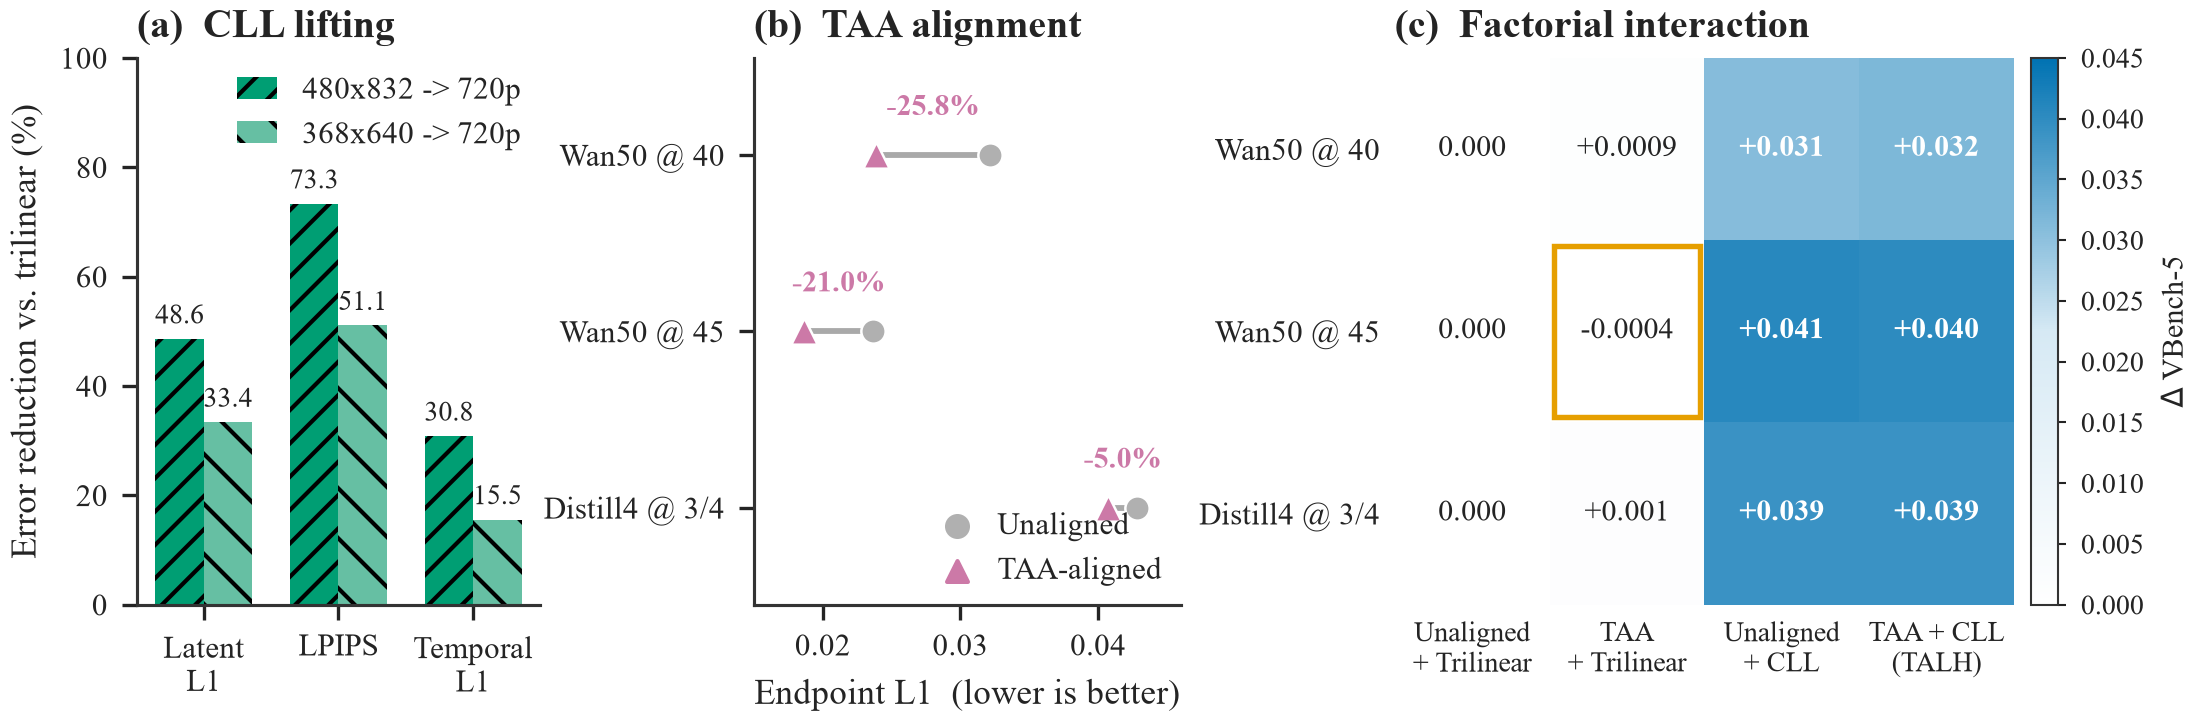
\includegraphics[width=\textwidth]{figures/fig_component_evidence.png}
\caption{Component evidence. (a) CLL outperforms trilinear lifting. (b) TAA reduces endpoint gaps on Wan50 and Distill4. (c) The factorial study attributes the dominant VBench-5 gain to CLL and local trajectory correction to TAA.}
\label{fig:components}
\end{figure*}

\subsection{Human Evaluation and Distilled Transfer}

Against the corresponding CLL-only output, TAA wins fine-detail votes on 8/10 prompts at step 40 and 9/10 at step 45, but loses temporal-stability votes on 9/10 and 8/10. TAA therefore favors sharper local detail with some frame-to-frame fluctuation. By contrast, TALH-E beats trilinear handoff on all ten prompts for artifacts, details, overall quality, and identity preservation, and on nine for temporal stability. The Supplement gives all votes and agreement statistics.

On Distill4, TAA reduces endpoint \(L_1\)/LPIPS by 5.03\%/5.65\% on every paired sample, and TALH-D4 raises VBench-5 from 0.81796 (trilinear) to 0.85680 while changing latency from 167.09 to 170.29 seconds. Spatial handoff thus composes with temporal step distillation.

\subsection{Qualitative Comparison}

Figure~\ref{fig:teaser}(a) compares trilinear, CLL-only, and TALH-Q on content-aligned frames. CLL restores high-frequency texture, while TAA makes localized corrections. Native-HR (estimated) is the content-aligned complete 368p trajectory shown at the target display size: true 720p Native-HR can generate different content under the same seed and is therefore used for the paired quantitative evaluation in Table~\ref{tab:system}, not pixel-aligned crops. The Supplement provides additional spatial and temporal comparisons, including TALH-E.

\section{Discussion and Limitations}

The decomposition makes module roles measurable: TAA reduces scheduler- and step-dependent endpoint error, CLL learns a stable scale mapping, and HTR delegates texture synthesis to the frozen high-resolution prior. Model-endogenous supervision avoids external paired data and an additional teacher. However, CLL remains specific to the Wan VAE and generated-data distribution; downsampled clean latents and native low-resolution endpoints retain a distribution gap; fixed-step adapters do not yet support adaptive handoffs; and TALH is not a restoration method for compression, blur, or sensor noise. TAA's local improvements also need not produce monotonic aggregate VBench changes.

TALH inherits the content risks of its base generator. Deployment should retain the base model's licensing, safety filtering, and synthetic-media disclosure mechanisms.

\section{Conclusion}

TALH accelerates high-resolution video diffusion by pairing a low-resolution prefix with a high-resolution suffix and decomposing their handoff into TAA alignment, CLL lifting, and HTR re-entry. TALH-Q/E achieve \(1.83\times/2.22\times\) speedups while retaining 97.76\%/97.53\% of Native-HR VBench-5. CLL provides the dominant cross-scale gain, TAA consistently narrows residual endpoints, and both transfer to a four-step distilled sampler using supervision generated by the frozen target model itself.
